%************************************************
\chapter{Results}\label{p03:results}
%************************************************
In this chapter, experiments are performed to find the best implementation/settings of the algorithm. As explained in chapter \ref{p02:session_tracking}, a wrong value of the "session\_timeout" parameter can produce different and perhaps incorrect results.
First the session timeout for the reading sessions will be determined by trying and analyzing different parameter values. Second, a the session timeout for the exercise sessions will be determined.

\section{Reading session experiments}
The reading session tracking is the most complex to model, because there are multiple internal and external variables to consider. First, we must define what actions are relevant to detect, in order to consider them as part of the learning process, and which ones are not (\Ie\ the user trying to game the system). Second, with the events already defined, we must determine how much time can pass between them, which is still part of the same reading/learning session.

The set of \textbf{opening, interaction and closing events} were defined as listed in table \ref{tb:event_type_v1}.

\begin{table}[htb]
	\begin{tabularx}
		{\textwidth}{Xll}\toprule
		\tableheadline{Event} & \tableheadline{Action type} \\ 
		\midrule 
		ARTICLE CLOSED & Closing \\ 
		\hline 
		CHANGE ORIENTATION & Interaction \\ 
		\hline 
		CLOSE ALTERMENU & Interaction \\ 
		\hline 
		OPEN ALTERMENU & Interaction \\ 
		\hline 
		SEND SUGGESTION & Interaction \\ 
		\hline 
		SPEAK TEXT & Interaction \\ 
		\hline 
		TRANSLATE TEXT & Interaction \\ 
		\hline 
		UNDO TEXT TRANSLATION & Interaction \\ 
		\hline 
		ARTICLE FOCUSED & Opening \\ 
		\hline 
		OPEN ARTICLE & Opening \\ 
		\hline 
		OPEN STARRED ARTICLE & Opening \\ 
		\hline 
		ARTICLES REQUESTED FROM ZEEGUU & Closing \\ 
		\hline 
		SCROLL & Interaction \\ 
		\hline 
	\end{tabularx} 
	\caption{User events classification}\label{tb:event_type_v1}
\end{table}

\subsection{Baseline}
For the baseline an arbitary value of 5 minutes for the \textbf{session\_timeout} was used.

By observing the total reading time by user, we can see that the highest value is 2788 minutes (almost 2 days). By analyzing the daily activity for a specific user, we find long reading sessions spanning up to 1:20 hours long. Figure \ref{fig:visualizations_1st_iteration} show these results.

\begin{figure}[bth]
	\myfloatalign
	\subfloat[Total read time by user]
	{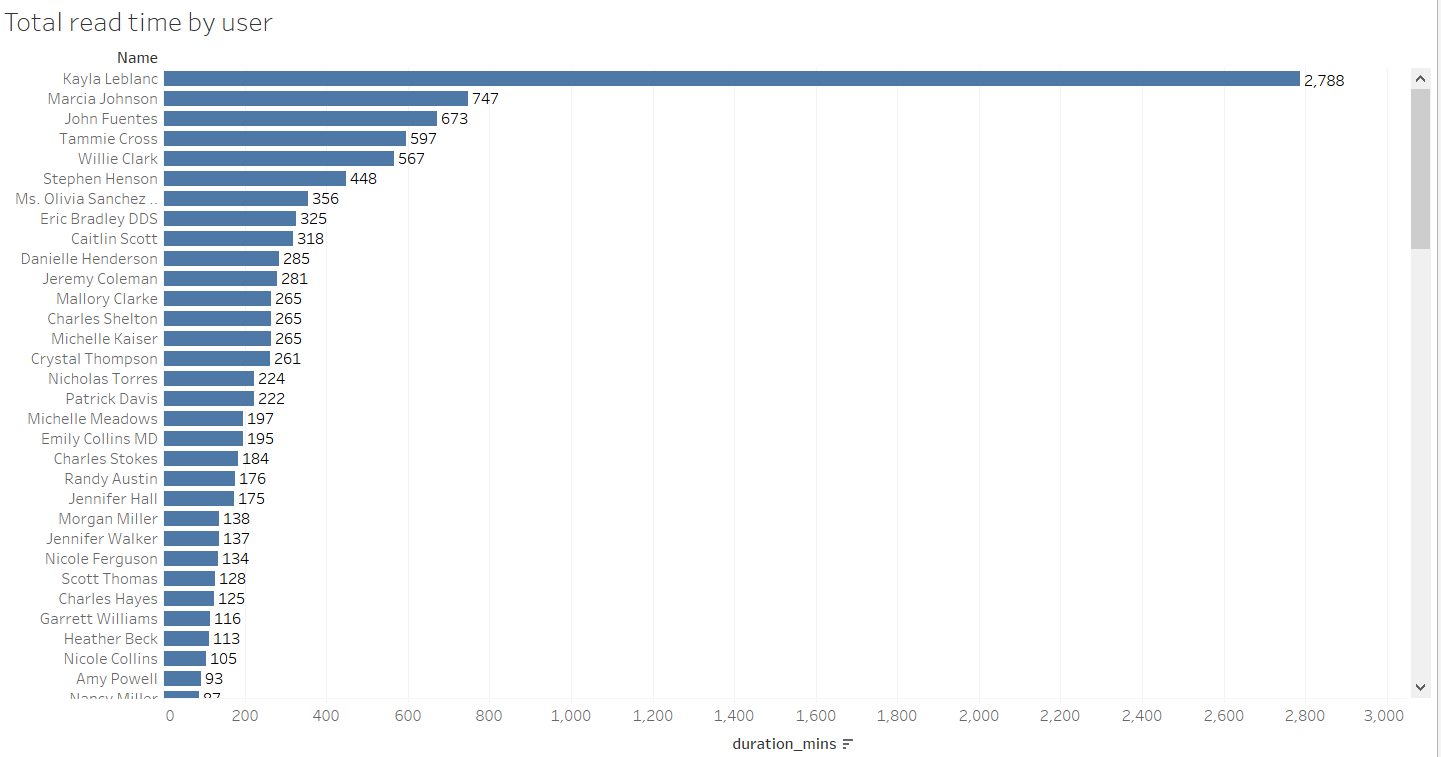
\includegraphics[width=1\linewidth]{gfx/total_read_time_by_user_5min}\label{fig:total_read_time_5min_no_scroll}} \quad 
	\subfloat[Daily activity timeline]
	{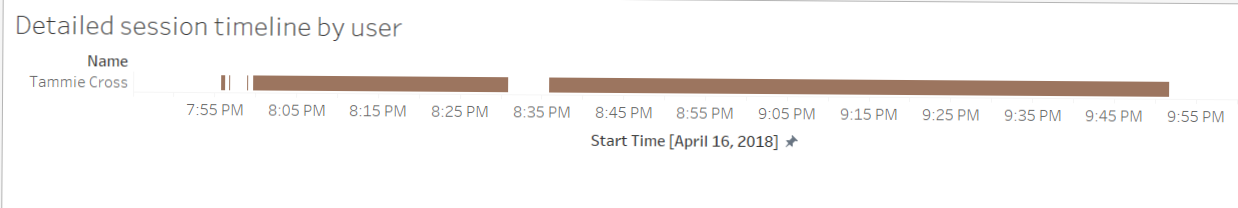
\includegraphics[width=1\linewidth]{gfx/detailed_session_timeline_by_user_5min_no_scroll}\label{fig:detailed_session_timeline_by_user_5min_no_scroll}} \quad
	\caption{Reading session visualizations for session\_timeout of 5 minutes.}\label{fig:visualizations_1st_iteration}
\end{figure}


\subsection{Improving the baseline}
Using the previous settings as a baseline, the next idea was to reduce the value of session\_timeout, because the additional time benefit of 5 minutes might be too much grace time for a user reading without doing any action. Scrolling events are helpful to detect more frequent activity, but they can be overwhelming for the web server and the database, for that reason, the web server callback was limited to maximum 1 call per minute.

Sessions were computed using different parameters for the session\_timeout, and the maximum idle time between user actions inside a session was plotted (figure \ref{fig:idle_time_comparison}).

\begin{figure}[bth]
	\myfloatalign
	\subfloat[1 min]
	{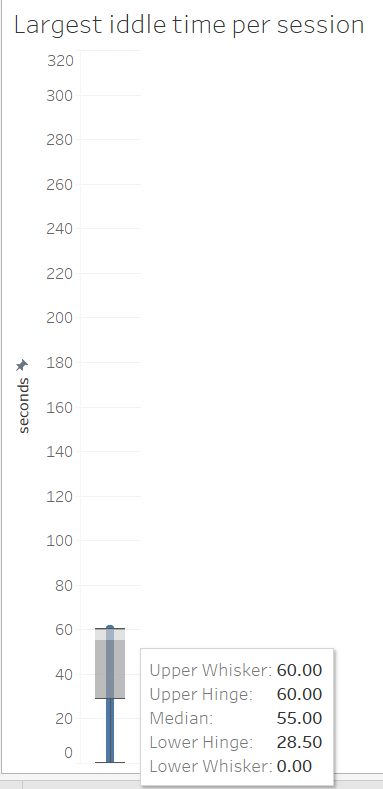
\includegraphics[width=0.19\linewidth]{gfx/largest_iddle_time_1min_timeout}\label{fig:largest_iddle_time_1min_timeout}}  
	\subfloat[2 min]
	{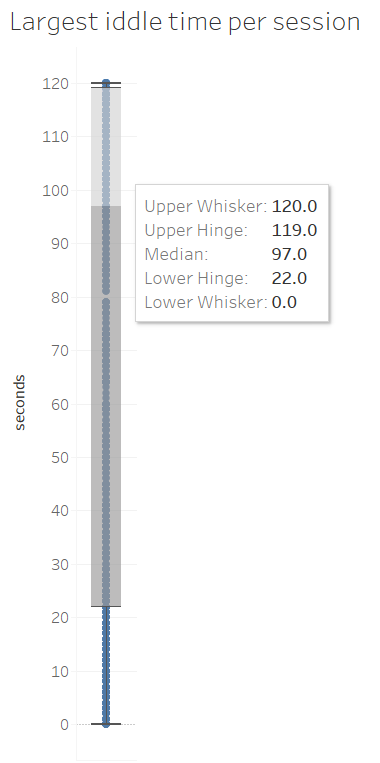
\includegraphics[width=0.19\linewidth]{gfx/largest_iddle_time_2min_timeout}\label{fig:largest_iddle_time_2min_timeout}} 
	\subfloat[3 min]
	{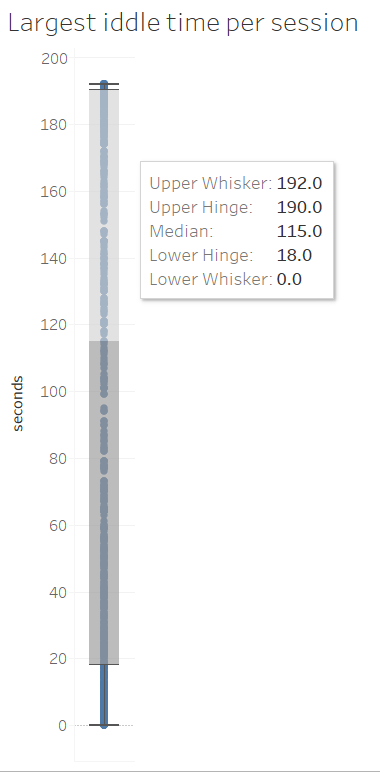
\includegraphics[width=0.19\linewidth]{gfx/largest_iddle_time_3o2min_timeout}\label{fig:largest_iddle_time_3o2min_timeout}}
	\subfloat[4 min]
	{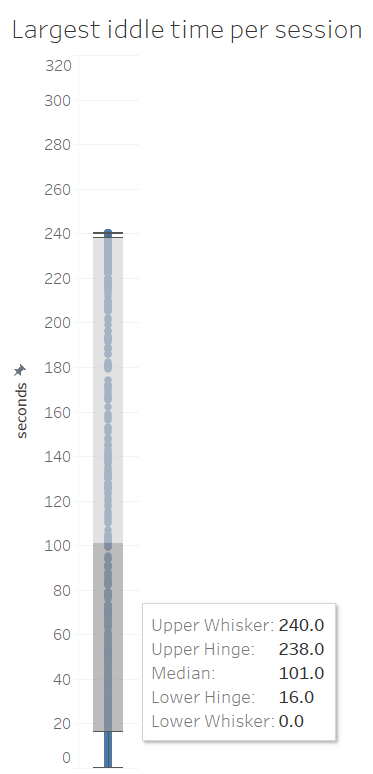
\includegraphics[width=0.19\linewidth]{gfx/largest_iddle_time_4min_timeout}\label{fig:largest_iddle_time_4min_timeout}} 
	\subfloat[5 min]
	{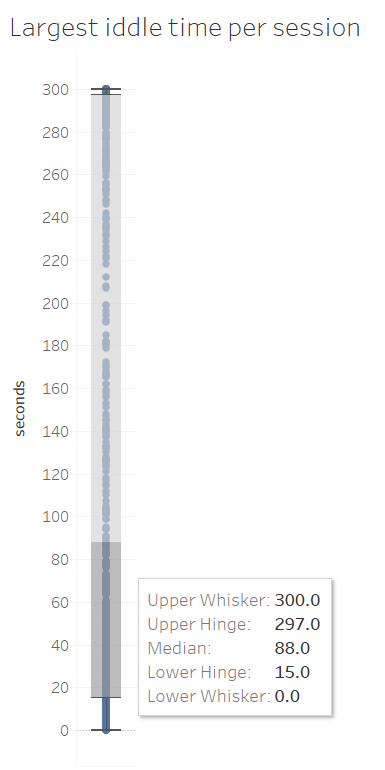
\includegraphics[width=0.19\linewidth]{gfx/largest_iddle_time_5min_timeout_v2}\label{fig:largest_iddle_time_5min_timeout_v2}} \quad
	
	\caption{Box plot of maximum idle time per session, for distinct session timeout values}\label{fig:idle_time_comparison}
\end{figure}

We can observe that the median value fluctuates between 90 and 120 seconds (as shown in table \ref{tb:table_median_value}). By taking this value into account and some empirical measures, the value of the timeout was set to 2 minutes. 

The upper hinge, however, increases as the timeout value do. This is because small sessions are stitched together, therefore moving the value upwards.

\begin{table}[htb]
	\begin{tabularx}
		{\textwidth}{Xllll}\toprule
		\tableheadline{Timeout value (min)} & 
		\tableheadline{Median (sec)} &
		\tableheadline{Upper hinge(sec)} \\ 
		\midrule 
		1 & 55 & 60 \\ 
		\hline 
		2 & 97 & 119 \\ 
		\hline
		3.2 & 115 & 190\\ 
		\hline 
		4 & 101 & 238\\ 
		\hline 
		5 & 88 & 297\\ 
		\hline 
	\end{tabularx} 
	\caption{Maximum idle time statistics with different session timeout values}\label{tb:table_median_value}
\end{table}

By comparing the total time per user between the baseline and the final settings (figure \ref{fig:total_time_comparison}), we can observe that a reduction of almost 300\% in the total time per user was achieved. This means that the previous session\_timeout value was too big, therefore computing times longer than what they really were.

\begin{figure}[!htb]
	\myfloatalign
	\subfloat[Baseline (5 minutes)]
	{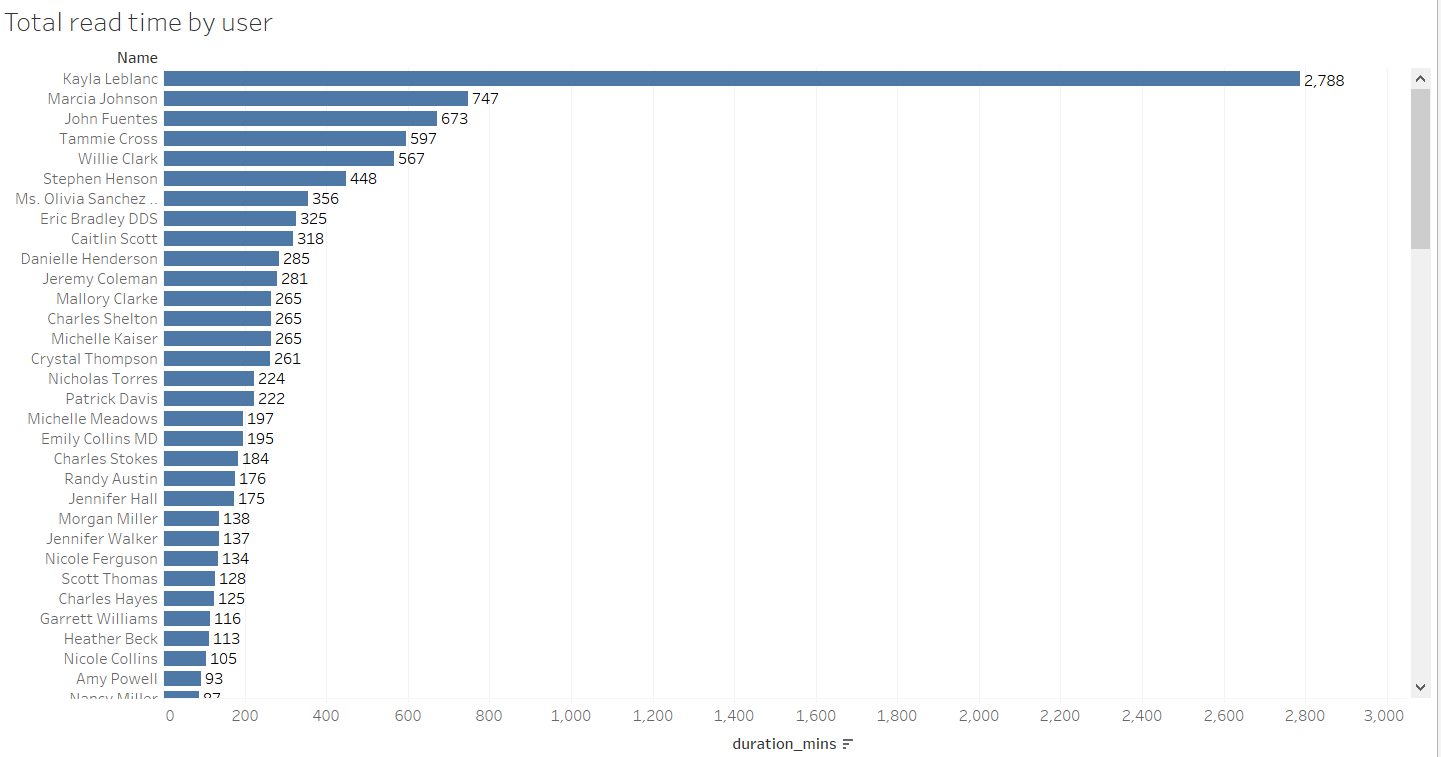
\includegraphics[width=1\linewidth]{gfx/total_read_time_by_user_5min}\label{fig:total_read_time_by_user_5min}} \quad 
	\subfloat[Final settings (2 minutes)]
	{
	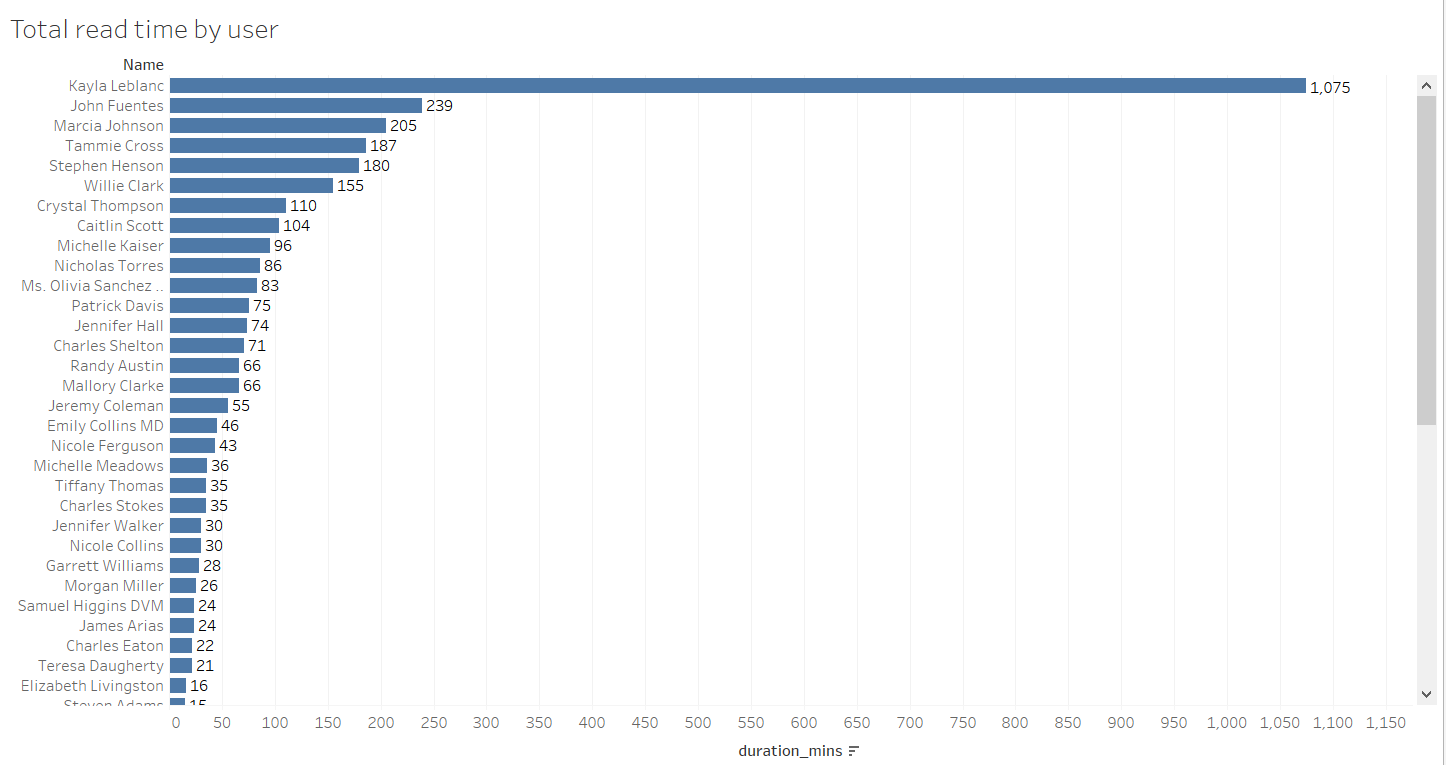
\includegraphics[width=1\linewidth]{gfx/total_read_time_by_user_2min}\label{fig:total_read_time_by_user_2min}} \\
	\caption{Total time improvement comparison}\label{fig:total_time_comparison}
\end{figure}

Finally, for the detailed activity, a big change is observed, in figure \ref{fig:detailed_session_5min}, we observe roughly two smooth reading sessions, which later, with a finer session detection gets split into smaller reading sessions (figure \ref{fig:detailed_session_2min}). This means that we correctly detected the user's gap of attentions, therefore a more precise session time was measured.

\begin{figure}[!htb]
	\myfloatalign
	\subfloat[Baseline (5 minutes)]
	{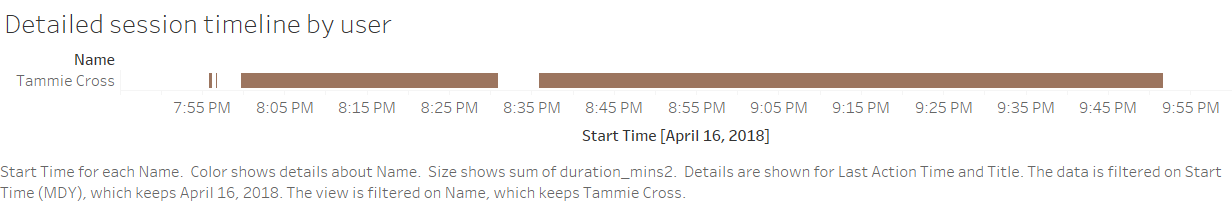
\includegraphics[width=1\linewidth]{gfx/detailed_session_timeline_by_user_5min}\label{fig:detailed_session_5min}} \quad 
		
	\subfloat[Final settings (2 minutes)]
	{
	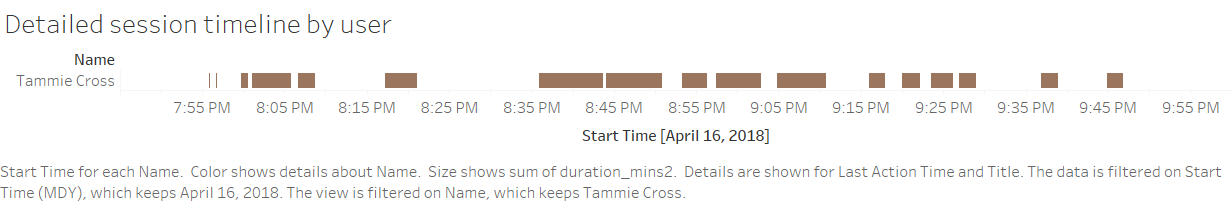
\includegraphics[width=1\linewidth]{gfx/detailed_session_timeline_by_user_2min}\label{fig:detailed_session_2min}} \\
	\caption{Low level session tracking time line}\label{fig:detailed_session_comparison}
\end{figure}

\section{Exercise session experiments}
For the exercise sessions, the implementation is quite simple. Only two events are tracked:
\begin{itemize}
	\item Answering the exercise (either right or wrong)
	\item Asking for a hint
\end{itemize}

The only parameter to define is the exercise session\_timeout. For the exercises, we know that they are short and quick activities, which take only a couple of second to provide an answer. Therefore the timeout must be much smaller than for reading.

In this case, the time between the exercise opening and the answering is computed by a timer. Therefore by a descriptive analysis of the answering time (box plot in figure \ref{fig:exercise_solving_speed}). The obtained results are 6, 10 and 21 seconds, which represent the median, upper hinge and upper whisker. These metrics represent the 50\%, 75\% and 100\% of a normally distributed population. 

\begin{figure}[bth]
	\centering
	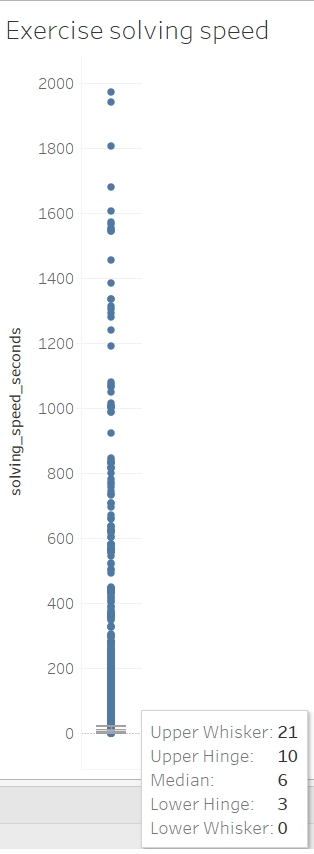
\includegraphics[width=0.2\linewidth]{gfx/exercise_solving_speed}
	\caption{Exercise time box plot}\label{fig:exercise_solving_speed}
\end{figure}

Given that the tracked time window is so small, a final setup of no grace time but using the upper whisker value (21 seconds) is chosen.
